\section{System's Perspective}
  \subsection{System Design}
  The developed MiniTwit system is complex and consists of many subsystems, each of which required a significant amount of decisions to construct.
  In this subsection, we will describe the design of our system as a whole, including the rationale behind some of the decisions we have made during this project.
  \newline
  For the sake of clarity, we will dissect our system into three different layers: frontend, API and data persistence.
  \begin{enumerate}
    \item \textbf{Frontend}\newline
    The frontend of our system is what provides users access to our system through a web interface, which is developed using Blazor (wasm) and C\#, as well as html and css.
    With blazor we were able to have our C\# code compiled to webassembly and executed with near-native performance within the client browser.
    The frontend communicates with our API using HTTP requests, containing json payloads of serialized or deserialized data.
    Apart from communicating with the REST API, the frontend also communicated directly with the RabbitMQ broker to send and receive private messages.
    This communication took place over WSS using the MQTT protocol. MQTT communication was then bound to a message queue on the broker. 
    
    \item \textbf{API}\newline
    The REST API was developed using ASP.NET and exposes endpoints for communicating with the MiniTwit service. 
    This includes execution of actions like following and unfollowing, as well as data fetching like feeds or user profiles.
    The API translates frontend HTTP calls into data manipulations using Entity Framework for ORM with a code-first approach.
    This allowed us to focus on code first and automatically construct relational database schemas based on the relations between objects in our C\# code, managed by database migrations.
    Various metrics were also exposed on the API, allowing us to monitor the system externally.
    
    \item \textbf{Data Persistence}\newline
    For data persistence we used multiple different database management systems. 
    MiniTwit data such as users, followers and messages were stored in a Postgres relational database, which integrates well with Entity Framework.
    Logging data are stored in an ElasticSearch database configured with lifetime policies to keep the size under control.
    Lastly we used RabbitMQ for temporarily storing user private messages in message queues, interfaced by MQTT over WS, to allow direct communication from our blazor frontend.
  \end{enumerate}

  \subsection{System Architecture}
  Our system as a whole consisted of 3 servers and a load balancer, all of which were hosted on DigitalOcean.
  Each server is running an NGINX server, which has been configured to serve as a reverse proxy for routing of subdomain access, e.g. master.pythonkindergarten.tech, slave.pythonkindergarten.tech, monitor.pythonkindergarten.tech etc.
  \newline
  Below is an overview of the 3 servers, as well as their function and purpose within our system.\newline
  
  \begin{enumerate}
    \item \textbf{Master Server}\newline
    The Master server was the master node in our Docker swarm and was responsible for maintaining cluster state, as well as managing service updates within the swarm.
    This server also hosted our Prometheus and Grafana containers, which were described in the monitoring section.
    \item \textbf{Worker Server}\newline
    The Worker server simply contributed to the pooled resources within our swarm. 
    It is a Docker swarm worker node, which ran multiple replicas of our service, hosting both API and frontend.

    \item \textbf{Database Server}\newline
    The Database server had multiple purposes, all of which related to data persistence.
    This server hosted our Postgres database, which was our primary means of persistence within the system. 
    \newline
    It also hosted our logging system, which consisted of an ElasticSearch database (for log persistence), as well as Kibana for visualization of the collected logs.
    \newline
    Lastly, it hosted our RabbitMQ broker.
    \item \textbf{Load Balancer}\newline
    The load balancer was hosted on Digital Ocean and allowed us to balance incoming traffic on pythonkindergarten.tech between each of our docker swarm servers.
  \end{enumerate}
  \subsubsection{System Deployment}
  We have automated deployment of our MiniTwit system using Terraform and bash scripts.
  Terraform enabled us to automate the following parts of our deployment:\newline

  \textbf{Startup and configuration of:}
  \begin{itemize}
    \item Master nodes
    \item A leader node
    \item A DigitalOcean load balancer
    \item The creation of a floating ip
    \item Adding domain with DNS records pointing to our floating ip
    \item A database droplet running a Postgres database, an ELK stack (without the L but replaced by Serilog), Prometheus and Kibana
  \end{itemize}
  
  Due to the high setup/configuration complexity, some parts of the system were left unconfigured after the automated deployment.
  This included the following parts of our system:\newline
  
  \textbf{The configuration of:}
  \begin{itemize}
    \item Prometheus (scrape targets)
    \item Grafana (dashboards, data sources and administration login)
    \item Kibana (dashboards, index creation, Index Lifecycle Management)
    \item Nginx (reverse proxy)
  \end{itemize}
  
  

  \subsection{Subsystem interactions}
  There are many important subsystems (described in previous sections), collectively making the system work as a whole.
  In this section we will illustrate the most important interactions between these services, as seen in the diagram below.\newline

\newpage

\begin{figure}[h!]
    \centering
    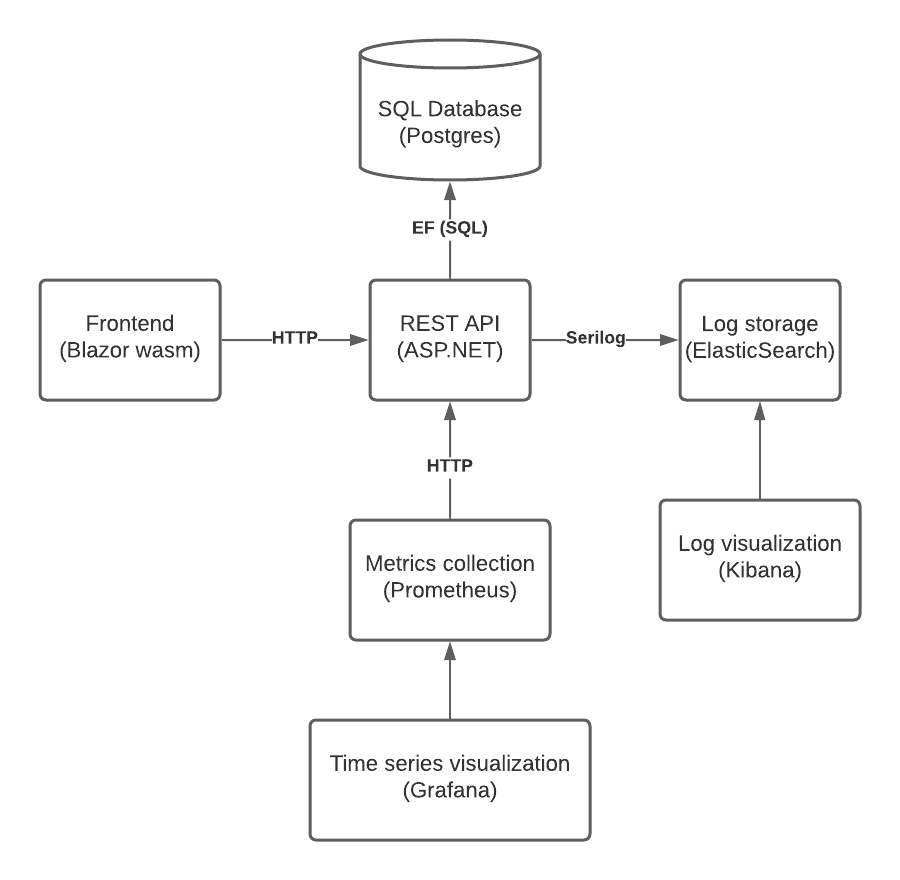
\includegraphics[scale=0.7]{images/InteractionDiagram.png}
    \caption{ Overview of Subsystems Interactions }
\end{figure}  

\subsection{Dependencies}
Below is a list of all the \textbf{dependencies} of the Pythonkindergarten MiniTwit project, classified by description:
\begin{itemize}
    \item \textbf{Language, Runtimes, Templates and Dependency Manager:}
      .Net 5.0, ASP.Net Runtime 5.0, Blazor WebAssembly, WASM, NuGet
    \item \textbf{Project Structure:} Server, Client, Shared, Tests
    \item \textbf{Database:} Postgres, EntityFramework Core, EntityFramework NPSQL
    \item \textbf{Testing:} Xunit
    \item \textbf{Repository and Distributed Version Control:} Github, Git
    \item \textbf{Domain names and Domain service:} Pythonkindergarten.tech, .Tech Domains
    \item \textbf{Data Transferring over HTTP:} JSON, System.Text.Json
    \item \textbf{Containerization:} Docker, Docker-Compose, DockerHub, Docker Swarm
    \item \textbf{Pipelines (CI/CD):} Github Actions (N.B. was initially Travis until migration to Github Actions)
    \item \textbf{Deployment Provider:} DigitalOcean
    \item \textbf{SSL Certificate for application:} ZeroSSL
    \item \textbf{Monitoring Tools:} Prometheus, Grafana
    \item \textbf{Virtualization:} Vagrant
    \item \textbf{Logging:} Elasticsearch, Serilog, Kibana
    \item \textbf{Static Codecheck Tools:} SonarScanner, SonarCloud, CodeQL
    \item \textbf{Messaging:} RabbitMQ
    \item \textbf{Infrastructure Deployment:} Terraform
\end{itemize}


\subsection{The current state of your system}
We used two different code analysis tools and they were both executed within our CI pipeline. 
The first one was SonarCloud, which analysed the API and WebAssembly projects for security issues, possible bugs and general code smells.

\begin{figure}[h!]
    \centering
    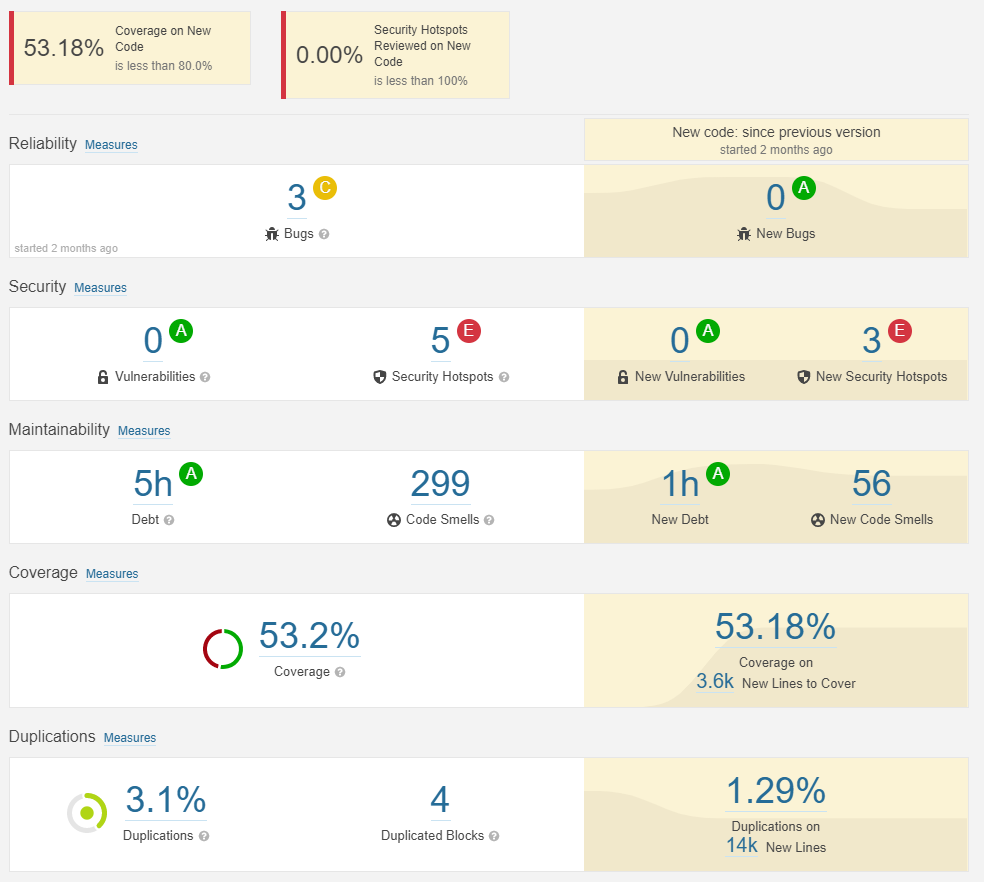
\includegraphics[scale=0.5]{images/sonar_latest_report.PNG}
    \caption{The latest report on static code analysis from Sonar Cloud}
\end{figure}

This tool showed that our test coverage was ~50\%, which was below SonarCloud's default expectation of 80\% and 90\%.

Other than that a lot of informational messages were present under the category "Code Smells". %CHECK UNTIL NEXT SCAN%

Additionally, there were a few informational security messages, which we looked through. 
However, they did not need to be acted on, because they were all false positives. 
Reports on "bad" exception handling also appeared, for example, by throwing top level exceptions eg. Exception. 

The second tool we used was called CodeQL, which was used to assess the security of our project. 
For example, hard coded credentials or other vulnerable data, which definitely shouldn't be visible to the public. 
Nothing of concern was found here, just false positives in our testing suite.

\newpage

\subsection{Licensing}
% Finally, describe briefly, if the license that you have chosen for your project is actually compatible with the licenses of all your direct dependencies. %

We have agreed to use the Apache 2.0 License for our application in order to have the highest degree of compatibility with our direct dependencies. 
To ensure that we have not violated any patents on our dependencies, we chose the most permissive of licenses. 

This license allows anyone to modify our software and to redistribute it, without any obligations to pay royalties.
